%--------------------------------------------------------------------
%--------------------------------------------------------------------
% Formato para los talleres del curso de Métodos Computacionales
% Universidad de los Andes
%--------------------------------------------------------------------
%--------------------------------------------------------------------

\documentclass[11pt,letterpaper]{exam}
\usepackage[utf8]{inputenc}
\usepackage[spanish]{babel}
\usepackage{graphicx}
\usepackage{tabularx}
\usepackage[absolute]{textpos} % Para poner una imagen en posiciones arbitrarias
\usepackage{multirow}
\usepackage{float}
\usepackage{hyperref}
%\decimalpoint

\begin{document}
\begin{center}
{\Large Métodos Computacionales} \\
\textsc{Tarea 2}\\
01-2019\\
\end{center}

\noindent
\section{Ejercicio 1: Fourier}
\subsection{Gráfica señales}
\begin{figure}[H]
\centering
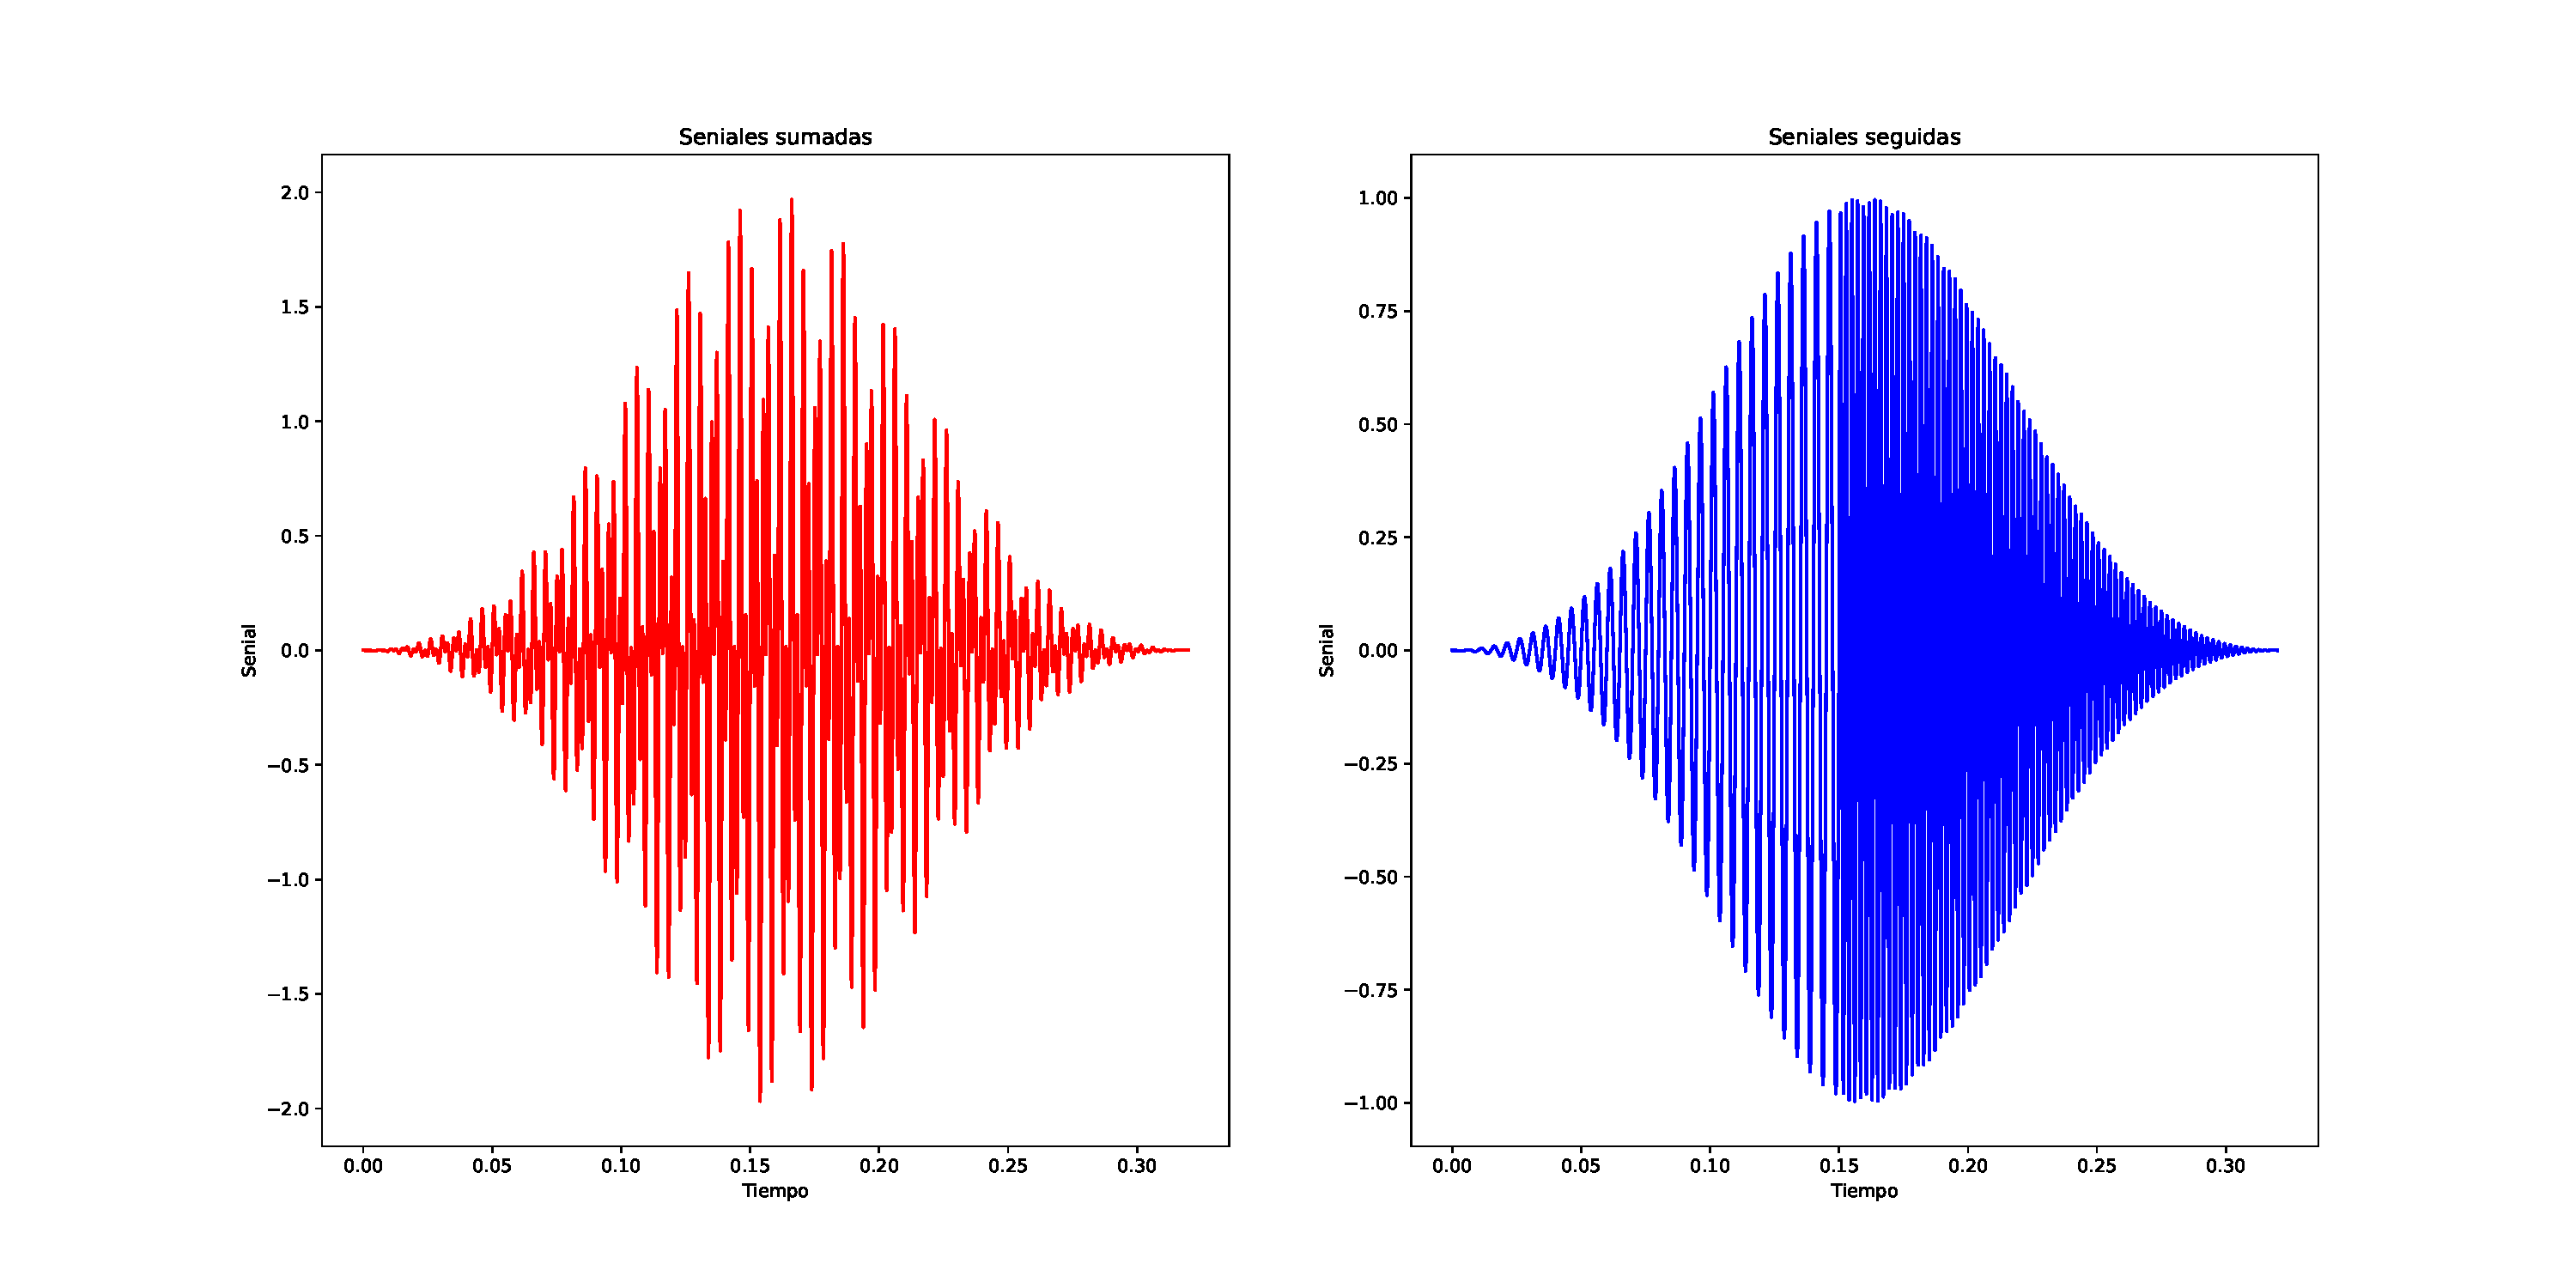
\includegraphics[scale=0.35]{PlotFourier1.pdf}
\end{figure}

\subsection{Gráfica señales transformadas}
\begin{figure}[H]
\centering
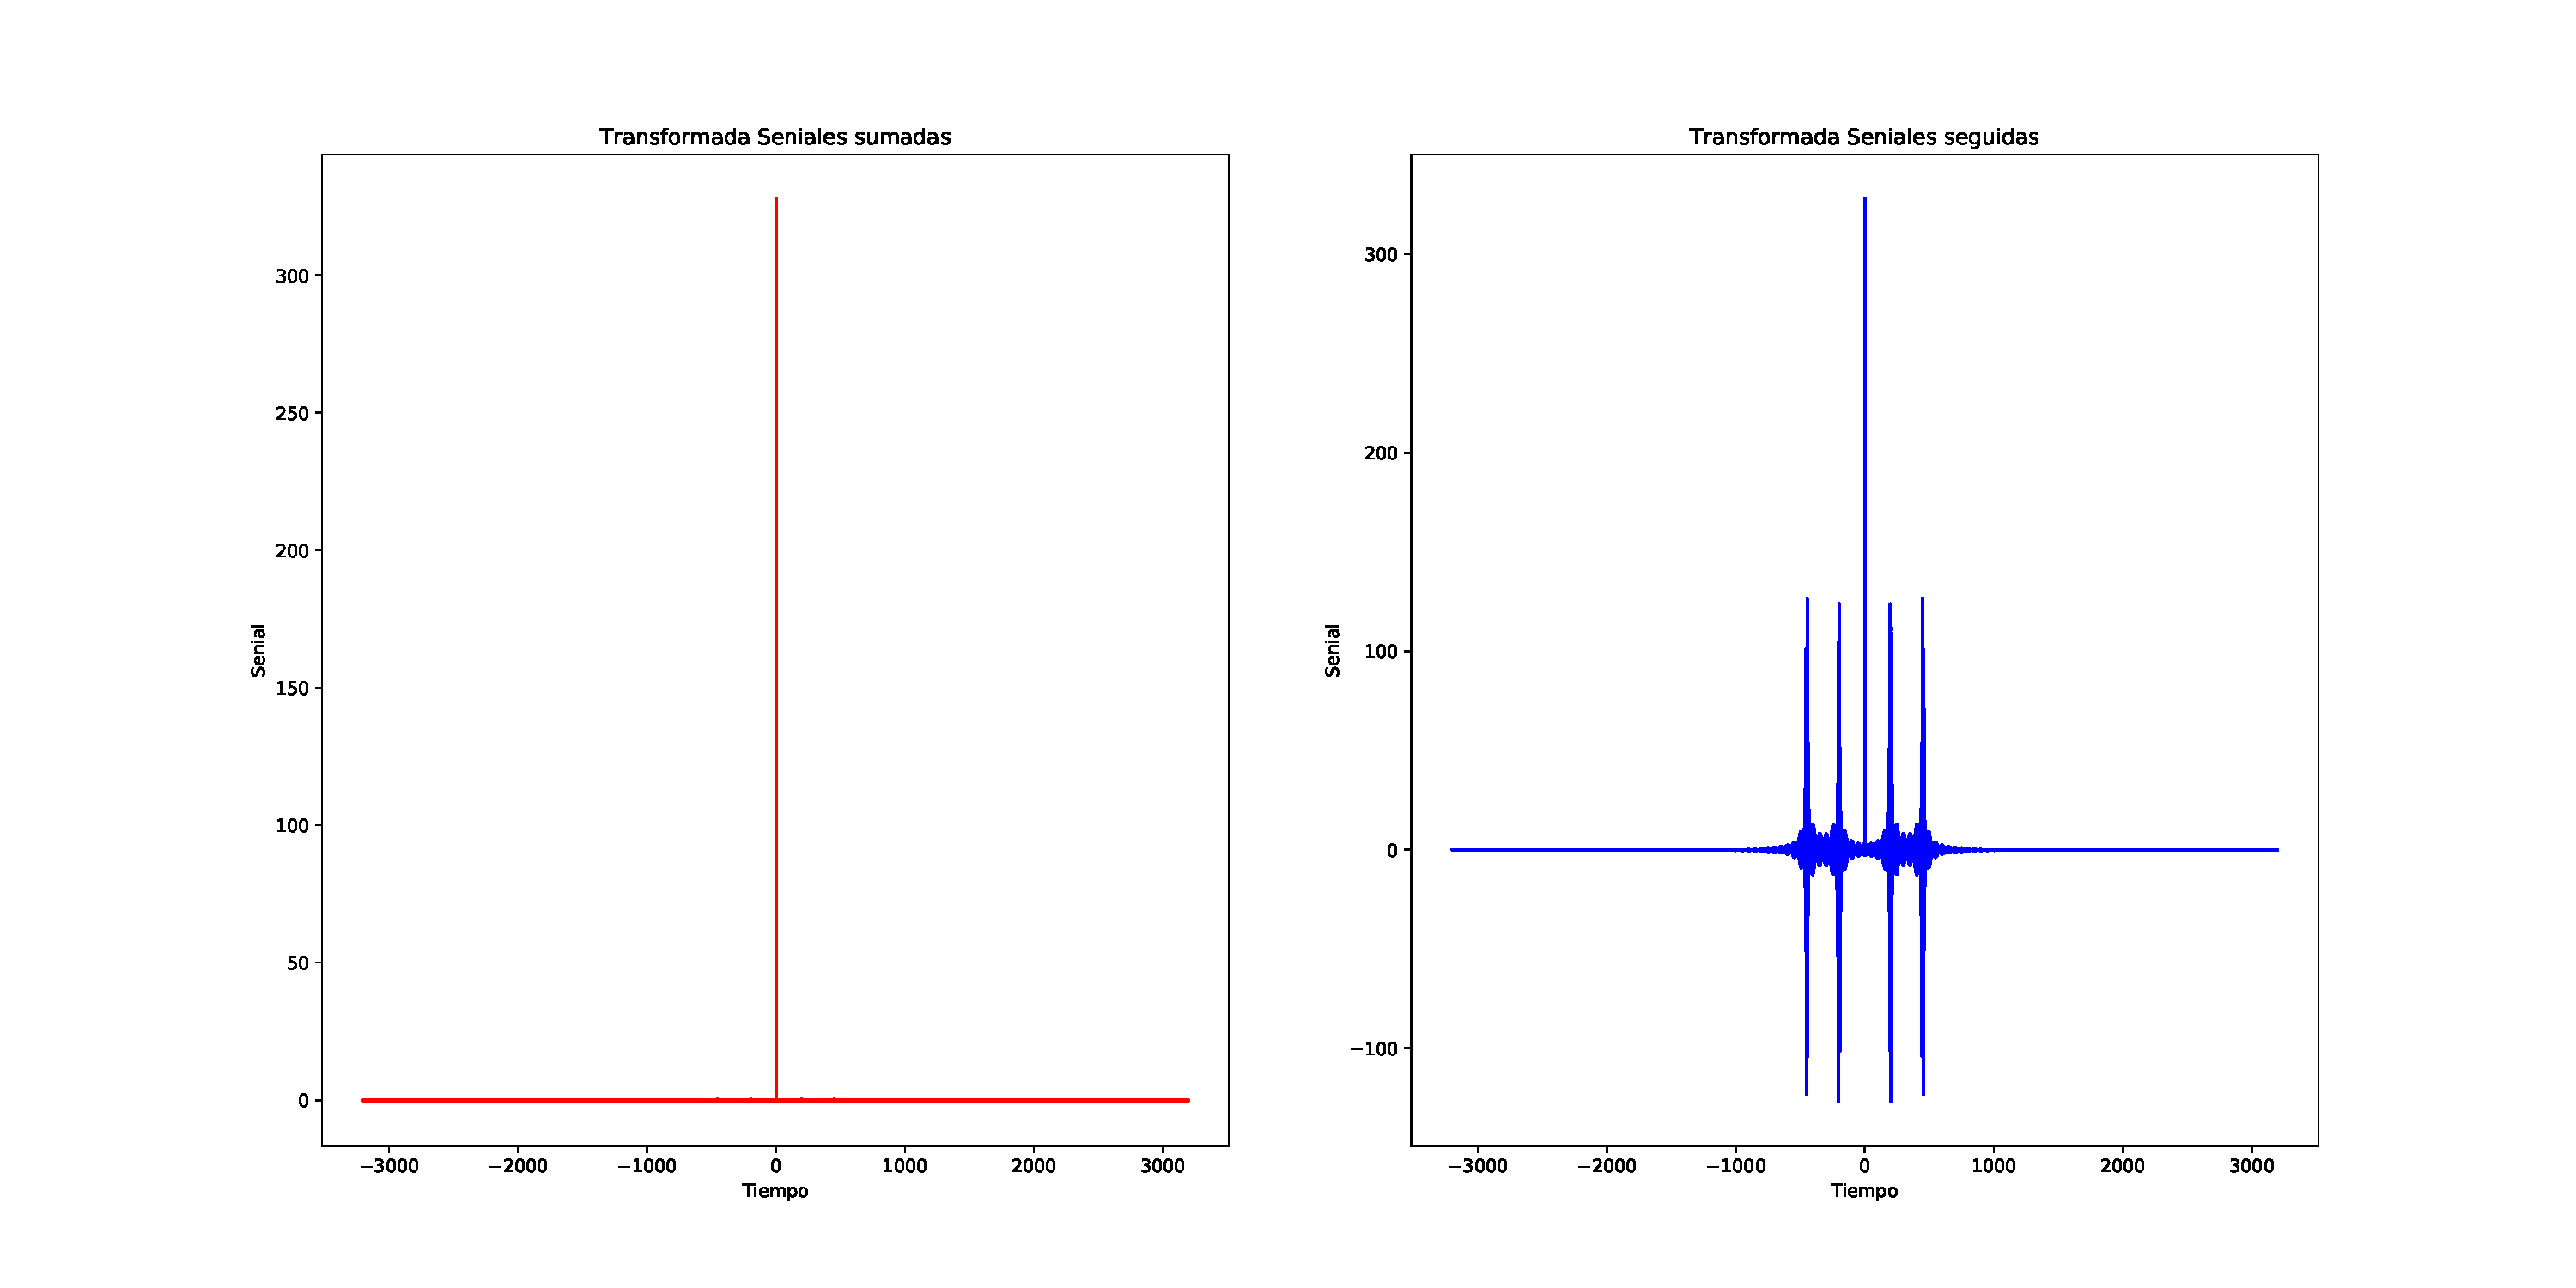
\includegraphics[scale=0.35]{PlotTransFourier2.pdf}
\end{figure}


\subsection{Espectrograma señal sumada}
\begin{figure}[H]
\centering
\includegraphics[scale=0.75]{specgram1.pdf}
\end{figure}

\subsection{Espectrograma señal seguida}
\begin{figure}[H]
\centering
\includegraphics[scale=0.75]{specgram2.pdf}
\end{figure}

\subsection{Gráfica señal temblor}
\begin{figure}[H]
\centering
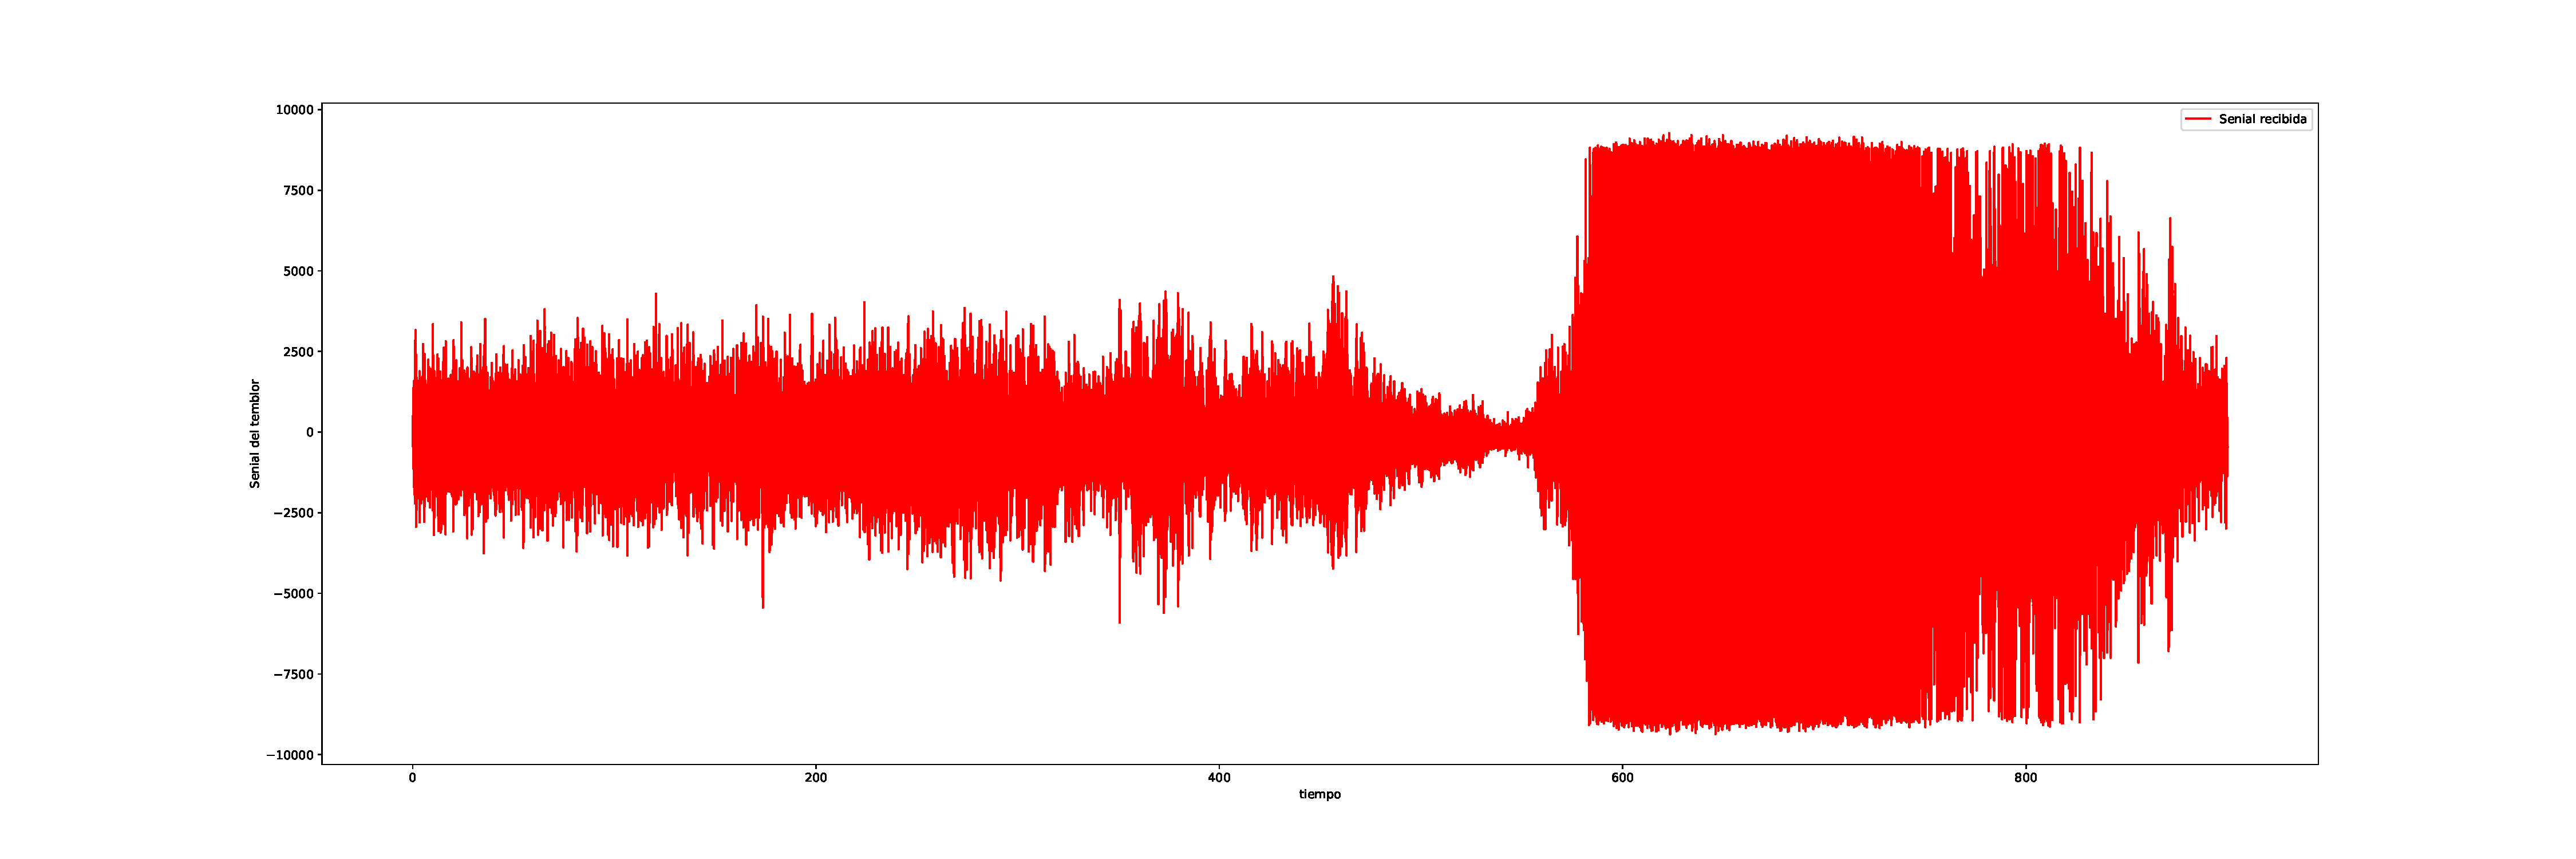
\includegraphics[scale=0.25]{PlotFourier3.pdf}
\end{figure}

\subsection{Gráfica señal temblor transformada}
\begin{figure}[H]
\centering
\includegraphics[scale=0.25]{PlotFourier4.pdf}
\end{figure}

\subsection{Espectrograma señal temblor}
\begin{figure}[H]
\centering
\includegraphics[scale=0.75]{specgramTemblor.pdf}
\end{figure}

\section{Ejercicio 2: ODEs}
\subsection{Amplitudes maximas en función de la frecuencia}
\begin{figure}[H]
\centering
\includegraphics[scale=0.4]{U_vs_freq.pdf}
\end{figure}

\end{document}
